\documentclass[11pt,a4paper]{article}
\usepackage[T5]{fontenc}
\usepackage[utf8]{inputenc}
\usepackage[vietnamese]{babel}
\usepackage{lmodern}
\usepackage[margin=2.3cm]{geometry}
\usepackage{amsmath,amssymb}
\usepackage{booktabs,tabularx,array}
\usepackage{enumitem}
\usepackage{float}
\usepackage{xcolor}
\usepackage{graphicx}
\usepackage{makecell}
\usepackage[numbers,sort&compress]{natbib}
\usepackage[hidelinks]{hyperref}
\setlist{itemsep=2pt,topsep=3pt}
\setlength{\emergencystretch}{2em}
\newcolumntype{L}{>{\raggedright\arraybackslash}X}
\newcommand{\sv}{\textsc{ViLexTime}}

\title{\textbf{Thesis}}
\author{}
\date{}

\begin{document}
\maketitle

% =====================================================================
\section{Abstract}
\begin{description}[leftmargin=0pt]
  \item[Title.] Truy xuất tăng cường dựa trên đồ thị tri thức có nhận biết thời gian cho hỏi đáp pháp luật Việt Nam theo mốc hiệu lực.

  \item[Context.] Văn bản quy phạm pháp luật Việt Nam thường xuyên được sửa đổi, bổ sung, thay thế hoặc bãi bỏ. Vì vậy, nội dung của cùng một quy định có thể khác nhau tùy thời điểm áp dụng, và câu trả lời đúng cho một câu hỏi pháp lý chỉ xác định được khi gắn với một mốc thời gian cụ thể. Chẳng hạn, khoản 2 Điều 61 Nghị định 142/2017/NĐ-CP quy định xử phạt vi phạm hành chính trong lĩnh vực hàng hải quy định thẩm quyền của Giám đốc Cảng vụ hàng hải, trong đó điểm b ban đầu cho phép phạt tiền đến 25.000.000 đồng. Điểm b khoản 37 Điều 1 Nghị định 123/2021/NĐ-CP đã sửa khoản này, nâng mức phạt tiền tối đa lên 50.000.000 đồng, có hiệu lực từ ngày 01/01/2022. Do đó, với cùng câu hỏi ``Giám đốc Cảng vụ hàng hải được phạt tiền tối đa bao nhiêu?'', đáp án theo quy định có hiệu lực tại ngày 16/02/2020 là 25.000.000 đồng, còn tại ngày 19/07/2022 là 50.000.000 đồng. Một hệ thống hỏi đáp pháp luật vì thế phải xác định được phiên bản quy định có hiệu lực tại thời điểm được hỏi, chứ không chỉ tìm đúng điều khoản liên quan.

  \item[Gap.] Các hệ thống sinh câu trả lời tăng cường truy xuất (RAG) hiện nay xếp hạng căn cứ theo mức độ liên quan với câu hỏi, không theo hiệu lực tại mốc được hỏi; vì vậy chúng có thể tìm đúng điều khoản nhưng trích lời văn của một phiên bản không có hiệu lực. Các tiếp cận dựa trên đồ thị như GraphRAG và LightRAG mô hình hóa quan hệ giữa các thực thể, nhưng không mô hình hóa hiệu lực theo thời gian. Trong phạm vi các tài liệu đã khảo sát, chưa có bộ dữ liệu hỏi đáp pháp luật tiếng Việt nào đánh giá câu trả lời theo phiên bản quy định có hiệu lực tại mốc thời gian của câu hỏi.

  \item[Solution.] Ý tưởng cốt lõi của đề tài là xác định trước phiên bản nào của mỗi quy định có hiệu lực vào thời điểm nào, rồi chỉ cho hệ thống truy xuất những phiên bản có hiệu lực tại mốc được hỏi. Giải pháp gồm ba thành phần. \emph{Thứ nhất}, lịch sử văn bản pháp luật được biểu diễn bằng một đồ thị pháp lý theo thời gian: mỗi nút là một Điều, Khoản hoặc Điểm; mỗi cạnh là một sự kiện sửa đổi hoặc bãi bỏ kèm ngày có hiệu lực. \emph{Thứ hai}, đồ thị này được biên dịch trước (offline) thành một kho phiên bản, trong đó mỗi điều khoản có một chuỗi phiên bản lời văn và mỗi phiên bản có một khoảng hiệu lực xác định. Khoảng hiệu lực này tính đến cả hiệu lực của Điều chứa khoản và của văn bản chứa điều. \emph{Thứ ba}, khi nhận một câu hỏi kèm mốc thời gian, hệ thống loại các phiên bản không có hiệu lực tại mốc đó ngay trong bước truy xuất, trước khi xếp hạng; mô hình ngôn ngữ vì vậy chỉ nhận được căn cứ hợp lệ, thay vì phải tự chọn phiên bản dựa trên ngày tháng được cung cấp. Để đánh giá giải pháp, đề tài xây dựng bộ dữ liệu \sv{}, trong đó mỗi câu hỏi gắn với một mốc thời gian và đáp án chuẩn lấy từ phiên bản có hiệu lực tại mốc đó. Câu trả lời được chấm theo cách tương phản: chỉ được tính là đúng khi chứa nội dung của phiên bản đúng và không chứa nội dung chỉ có ở phiên bản khác.

  \item[Results.] Trên bộ kiểm tra cuối gồm 318 cặp câu hỏi--mốc, với cùng mô hình sinh GPT-4o mini, RAG phẳng trích nội dung của phiên bản không có hiệu lực ở 25,3--29,1\% số dòng mà các phiên bản có nội dung khác nhau. Khi được cung cấp sẵn phiên bản có hiệu lực tại mốc hỏi, mô hình sinh đạt Accuracy 0,956; khi được cung cấp phiên bản hiện hành, Accuracy chỉ còn 0,456. Hệ đề xuất nâng Accuracy từ 0,324 (RAG lai ghép) lên 0,667, tức tăng 0,343 (KTC 95\%: [0,283; 0,401]), và kết quả nhất quán qua hai lần chạy độc lập. Tỷ lệ cặp câu hỏi được trả lời đúng ở cả hai mốc thời gian tăng từ khoảng 0,07 lên khoảng 0,65, trong khi MRR hầu như không đổi (0,445 so với 0,456), cho thấy các thước đo truy xuất thông thường không phản ánh được lỗi trích sai phiên bản.
\end{description}

% =====================================================================
\section{Introduction}

\paragraph{Bối cảnh và động lực.} Câu hỏi pháp lý luôn gắn với một thời điểm áp dụng cụ thể, chẳng hạn thời điểm xảy ra hành vi vi phạm hoặc thời điểm giao kết hợp đồng. Vì văn bản pháp luật được sửa đổi, bổ sung và bãi bỏ theo thời gian, quy định đúng để giải quyết một sự việc là quy định có hiệu lực tại thời điểm đó, không nhất thiết là quy định hiện hành. Một hệ thống hỏi đáp trả lời theo phiên bản hiện hành cho một sự việc đã xảy ra trước khi quy định được sửa đổi sẽ đưa ra câu trả lời sai, dù vẫn trích dẫn đúng điều khoản. Loại lỗi này đặc biệt khó phát hiện: câu trả lời đúng chủ đề, đúng điều khoản và có căn cứ rõ ràng, chỉ sai ở phiên bản lời văn được áp dụng. Do đó, ngoài việc tìm đúng điều khoản, hệ thống còn phải xác định được phiên bản có hiệu lực tại thời điểm được hỏi.

\paragraph{Hiện trạng và hạn chế.} Các hệ thống RAG phổ biến, dù dùng truy xuất từ vựng như BM25 \citep{robertson2009bm25}, truy xuất dày đặc \citep{karpukhin2020dpr} hay kết hợp cả hai \citep{cormack2009rrf}, đều xếp hạng căn cứ theo mức độ liên quan với câu hỏi mà không xét đến hiệu lực của căn cứ tại thời điểm được hỏi. Các tiếp cận dựa trên đồ thị như GraphRAG \citep{edge2024graphrag} và LightRAG \citep{guo2025lightrag} bổ sung quan hệ giữa các thực thể trích xuất từ văn bản, nhưng đồ thị thực thể này cũng không mã hóa khoảng hiệu lực của từng lời văn. Gần đây, một số nghiên cứu trên pháp luật Đức \citep{prior2026oldfriend}, pháp luật liên bang Hoa Kỳ \citep{yao2026lawinforce} và pháp luật Thái Lan \citep{akarajaradwong2026nitibenchplus} đã cho thấy việc lọc căn cứ theo mốc thời gian cải thiện chất lượng hỏi đáp; do đó, lợi ích của thông tin thời gian tự thân không phải là phát hiện mới. Tuy nhiên, trong phạm vi các tài liệu đã khảo sát, còn hai khoảng trống. Thứ nhất, chưa có đánh giá định lượng nào về mức độ phổ biến của lỗi trích sai phiên bản đối với pháp luật Việt Nam. Thứ hai, các nghiên cứu trên chưa tách riêng đóng góp của từng mức thông tin thời gian, gồm ngày hiệu lực của văn bản, khoảng hiệu lực của từng phiên bản, hiệu lực lan truyền từ đơn vị cấp trên và việc duyệt đồ thị tại thời điểm truy vấn, trên cùng một tập dữ liệu.

\paragraph{Đề xuất.} Để lấp hai khoảng trống trên, chúng tôi đề xuất xác định trước hiệu lực của từng phiên bản lời văn, rồi chỉ cho hệ thống truy xuất những phiên bản có hiệu lực tại mốc được hỏi. Cụ thể, lịch sử sửa đổi và bãi bỏ của văn bản pháp luật được biểu diễn thành một đồ thị pháp lý theo thời gian, và đồ thị này được biên dịch offline thành một kho phiên bản, trong đó mỗi phiên bản có một khoảng hiệu lực xác định. Khi trả lời, các phiên bản không có hiệu lực tại mốc được hỏi bị loại ngay trong bước truy xuất. Hình~\ref{fig:solution} minh họa cách tiếp cận này qua một ví dụ cụ thể. Để xác định mức thông tin thời gian nào thực sự tạo ra cải thiện, chúng tôi đánh giá giải pháp bằng một thang cấu hình, trong đó mỗi bậc chỉ bổ sung một mức thông tin thời gian so với bậc trước, và mọi cấu hình dùng chung dữ liệu, prompt và mô hình sinh.

\begin{figure}[H]
\centering
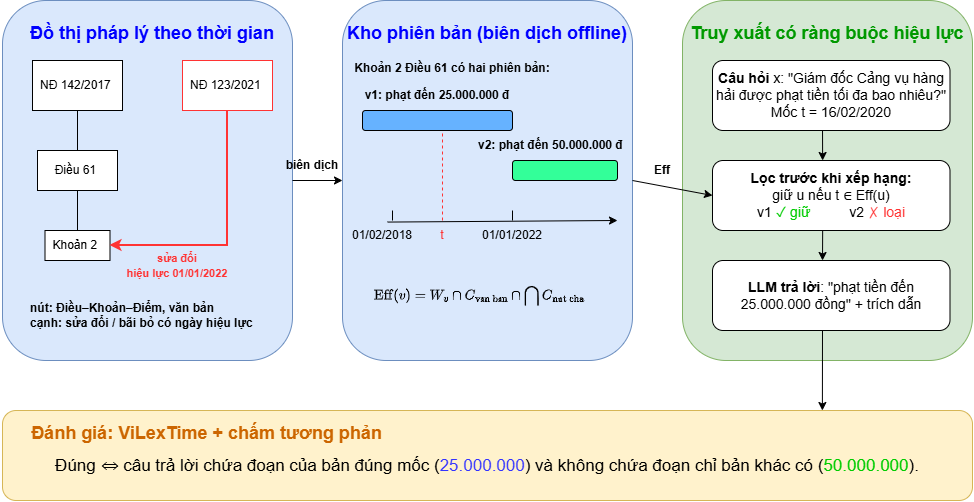
\includegraphics[width=\textwidth]{17_11.drawio.png}
\caption{Minh họa giải pháp bằng một ví dụ trong \sv{}. Đồ thị pháp lý theo thời gian ghi nhận cấu trúc văn bản và sự kiện sửa đổi có ngày hiệu lực; đồ thị được biên dịch offline thành chuỗi phiên bản với khoảng hiệu lực $\mathrm{Eff}(v)$. Khi truy vấn tại mốc $t$, phiên bản không có hiệu lực bị loại trước khi xếp hạng. Cách chấm tương phản phát hiện câu trả lời trích nội dung của phiên bản sai mốc.}
\label{fig:solution}
\end{figure}

\paragraph{Đóng góp.} Khóa luận có bốn đóng góp chính:
\begin{enumerate}
  \item \textbf{Kho phiên bản văn bản pháp luật Việt Nam.} Chúng tôi xây dựng quy trình dẫn xuất lịch sử lời văn của từng Điều, Khoản, Điểm từ các lệnh sửa đổi, bổ sung, thay thế và bãi bỏ thu thập trên cổng vbpl.vn. Kho thu được gồm 17.333 văn bản và 1.477.089 đơn vị phiên bản; khoảng hiệu lực của mỗi đơn vị được xác định có tính đến hiệu lực của các đơn vị cấp trên và của văn bản chứa nó.
  \item \textbf{Bộ dữ liệu \sv{}.} Chúng tôi xây dựng \sv{}, bộ dữ liệu hỏi đáp pháp luật tiếng Việt trong đó đáp án chuẩn của mỗi câu hỏi được gắn với phiên bản quy định có hiệu lực tại mốc thời gian của câu hỏi. Theo các tài liệu đã khảo sát, đây là bộ dữ liệu đầu tiên có đặc điểm này cho pháp luật Việt Nam. Mỗi điều khoản trong bộ dữ liệu được hỏi tại một hoặc nhiều mốc thời gian, ứng với các phiên bản lời văn khác nhau; bộ kiểm tra cuối gồm 361 câu hỏi kèm mốc thời gian, được xây dựng từ 199 điều khoản. Đi kèm bộ dữ liệu là phương pháp chấm tương phản, cho phép nhận diện câu trả lời trích nội dung của phiên bản không có hiệu lực, và hồ sơ ghi rõ nguồn gốc của từng nhãn.
  \item \textbf{Đánh giá theo kế hoạch phân tích được khai báo trước.} Chúng tôi so sánh mười hai cấu hình hệ thống và hai điều kiện oracle trên một bộ kiểm tra chưa từng được dùng trong quá trình phát triển. Các phép so sánh, thước đo và tiêu chí kết luận được cố định trước khi chạy thực nghiệm; mỗi hệ thống được chạy hai lần độc lập, và bảy phép kiểm định được hiệu chỉnh theo phương pháp Holm. Kết quả cho thấy, so với RAG lai ghép không sử dụng thông tin thời gian, hệ đề xuất tăng Accuracy thêm 0,343 và giảm tỷ lệ trích sai phiên bản 0,283, nhất quán ở cả hai lần chạy.
  \item \textbf{Phân tích nguồn gốc của cải thiện.} Chúng tôi phân tích thêm thành phần nào tạo ra cải thiện của hệ đề xuất. Đây là phân tích thăm dò, được thực hiện sau khi đã quan sát kết quả kiểm tra. Kết quả cho thấy phần lớn cải thiện đến từ việc kết hợp kho phiên bản với bộ lọc theo khoảng hiệu lực. Ngược lại, việc duyệt đồ thị tại thời điểm truy vấn không mang lại lợi ích đo được, và việc chỉ ghi ngày hiệu lực vào prompt cho mô hình ngôn ngữ cũng không thay thế được bộ lọc áp dụng trước khi xếp hạng.
\end{enumerate}

% =====================================================================
\section{Related Work}

\paragraph{Sinh câu trả lời tăng cường truy xuất và GraphRAG.} Sinh câu trả lời tăng cường truy xuất (RAG) kết hợp một bộ truy xuất với một mô hình sinh \citep{lewis2020rag}. Trong thực tế, truy xuất từ vựng như BM25 \citep{robertson2009bm25} và truy xuất dày đặc \citep{karpukhin2020dpr} thường được kết hợp, chẳng hạn bằng hợp nhất thứ hạng nghịch đảo (RRF) \citep{cormack2009rrf}. Các tiếp cận dựa trên đồ thị mở rộng hướng này: GraphRAG xây dựng đồ thị thực thể và tóm tắt theo cộng đồng cho các câu hỏi ở mức toàn kho \citep{edge2024graphrag}, còn LightRAG truy xuất trên đồ thị thực thể do mô hình ngôn ngữ trích xuất và mở rộng sang các nút lân cận \citep{guo2025lightrag}. Đối với văn bản luật, mạng nơ-ron đồ thị cũng đã được dùng để khai thác cấu trúc của bộ luật khi truy xuất điều khoản \citep{louis2023finding}. Điểm chung của các đồ thị này là chúng mô hình hóa thực thể hoặc cấu trúc, nhưng không mô hình hóa hiệu lực của một lời văn tại một thời điểm. Ngược lại, đồ thị trong khóa luận được xây dựng một cách tất định: nút là điều khoản và phiên bản, cạnh là sự kiện sửa đổi hoặc bãi bỏ có ngày hiệu lực.

\paragraph{Thời gian và phiên bản trong hỏi đáp.} TimeQA \citep{chen2021timeqa} và TempLAMA \citep{dhingra2022templama} đặt cùng một câu hỏi tại nhiều mốc khác nhau, nhưng cho tri thức miền mở. VersionRAG mô hình hóa phiên bản tài liệu trong miền tài liệu kỹ thuật \citep{huwiler2025versionrag}. Trong miền pháp luật, \citet{demartim2025satgraph} đề xuất đồ thị quy phạm có yếu tố thời gian dựa trên bản thể học; \citet{prior2025consolidation} cho thấy việc dùng mô hình ngôn ngữ để hợp nhất văn bản sửa đổi của Đức dễ phát sinh lỗi, và \citet{prior2026oldfriend} chỉ ra rằng bộ lọc theo mốc thời gian cải thiện đáng kể hỏi đáp luật thành văn. LawShift đánh giá dự đoán phán quyết khi luật thay đổi \citep{han2025lawshift}. Gần nhất với khóa luận, FiscalQA Pro xây dựng bộ đánh giá trên kho có phiên bản với cách chấm tất định cho luật thuế Pháp \citep{cymbler2026fiscalqa}, trong khi LawInForce-eCFR \citep{yao2026lawinforce} và NitiBench+ \citep{akarajaradwong2026nitibenchplus} lập chỉ mục các phiên bản có ngày và so sánh truy xuất có và không có thông tin thời gian. Các công trình này chưa tách riêng tác động của từng mức thông tin thời gian trên cùng một tập dữ liệu, và chưa có công trình nào cho pháp luật Việt Nam.

\paragraph{Hỏi đáp pháp luật tiếng Việt.} ALQAC tập trung vào truy xuất điều luật và suy diễn pháp lý \citep{thanh2021alqac}; VLQA \citep{nguyen2025vlqa}, VLegal-Bench \citep{dong2026vietlegal} và ViLegalExpert \citep{nguyen2026vilegalexpert} mở rộng quy mô và phạm vi tác vụ; ViHERMES nghiên cứu hỏi đáp đa bước trên văn bản quy định y tế với bộ truy xuất có nhận biết đồ thị \citep{nguyen2026vihermes}. Trong các phần tài liệu mà chúng tôi tiếp cận được, chưa bộ dữ liệu nào gắn đáp án chuẩn với phiên bản quy định có hiệu lực tại mốc thời gian của câu hỏi.

% =====================================================================
\section{Problem Formulation \& Methodology}

Hình~\ref{fig:overview} trình bày tổng quan phương pháp, gồm ba phần: biên dịch offline đồ thị pháp lý thành kho phiên bản, truy xuất có ràng buộc hiệu lực tại thời điểm truy vấn, và bộ dữ liệu \sv{} dùng để đánh giá.

\begin{figure}[H]
\centering
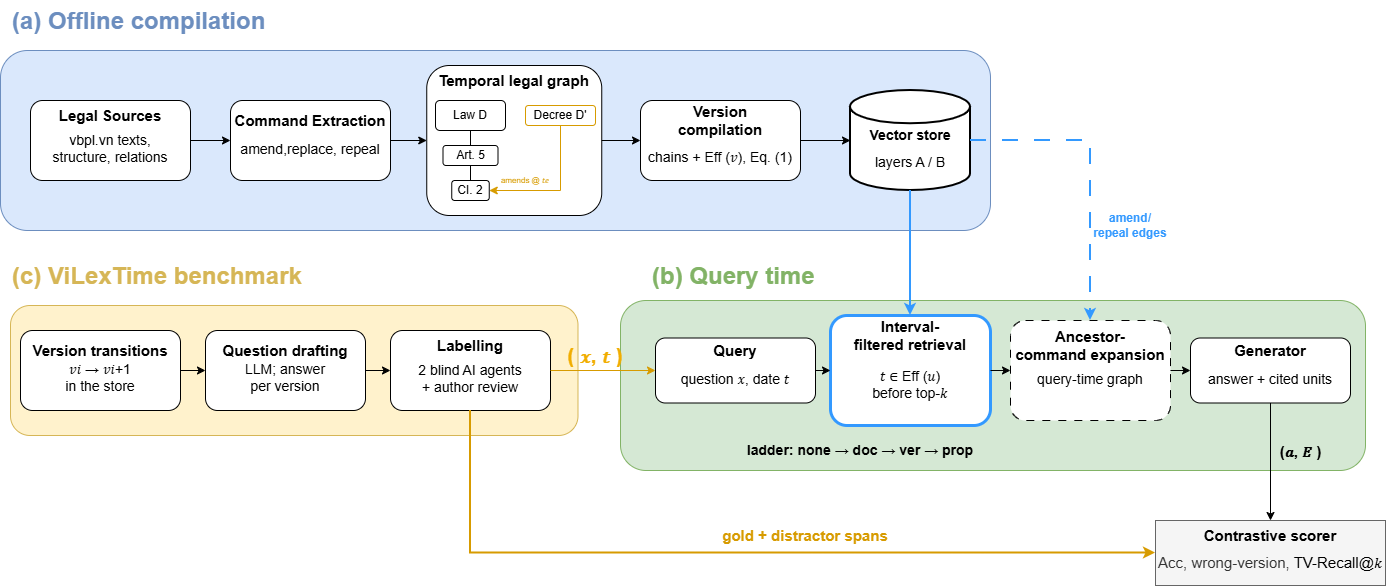
\includegraphics[width=\textwidth]{Fig2.drawio.png}
\caption{Tổng quan phương pháp. (a)~Lệnh sửa đổi và bãi bỏ được trích xuất thành cạnh có ngày hiệu lực trên cây cấu trúc văn bản, sau đó được biên dịch offline thành kho phiên bản kèm khoảng hiệu lực. (b)~Tại thời điểm truy vấn, các đơn vị không có hiệu lực tại $t$ bị loại trước khi chọn top-$k$; cấu hình đầy đủ bổ sung các lệnh tác động lên đơn vị cấp trên và kiểm tra trích dẫn. (c)~Bộ dữ liệu \sv{} cung cấp câu hỏi kèm mốc thời gian, cùng đoạn đáp án đúng và đoạn đáp án của phiên bản khác cho bộ chấm tương phản.}
\label{fig:overview}
\end{figure}

\subsection{Định nghĩa bài toán}
Cho một câu hỏi pháp lý $x$ bằng tiếng Việt và một mốc thời gian áp dụng $t$. Hệ thống cần trả về câu trả lời $a$ cùng tập căn cứ $E$ gồm các đơn vị pháp lý ở cấp Điều, Khoản hoặc Điểm, sao cho mọi căn cứ đều có hiệu lực tại $t$:
\begin{equation}
(x,t)\longmapsto(a,E),\qquad E\subseteq U,\quad \forall u\in E:\ \mathrm{valid}(u,t),
\label{eq:task}
\end{equation}
trong đó $U$ là tập đơn vị pháp lý trong kho. Nếu tại $t$ không còn quy định nào có hiệu lực điều chỉnh nội dung được hỏi, chẳng hạn do điều khoản đã bị bãi bỏ, hệ thống phải khẳng định rõ điều này; câu trả lời từ chối hoặc ``không biết'' không được xem là đúng. Mỗi cặp $(x,t)$ là một dòng dữ liệu; các dòng cùng thuộc một điều khoản được xem là phụ thuộc nhau và được lấy mẫu lại cùng nhau khi kiểm định.

\subsection{Biểu diễn phiên bản và khoảng hiệu lực}
Chúng tôi tách danh tính của một điều khoản $p$ khỏi lời văn của nó. Mỗi phiên bản $v$ của $p$ mang một lời văn có hiệu lực trên khoảng cục bộ nửa mở $W_v=[s_v,e_v)$. Khoảng cục bộ không đủ để xác định hiệu lực: một khoản có Điều chứa nó bị bãi bỏ, hoặc thuộc văn bản đã hết hiệu lực, thì không còn hiệu lực dù lời văn của chính khoản đó chưa từng bị sửa. Do đó, khoảng hiệu lực thực tế được tính trước (offline) như sau:
\begin{equation}
\mathrm{Eff}(v)=W_v\;\cap\;C_{\mathrm{doc}(p)}\;\cap\bigcap_{a\in\mathrm{anc}(p)}C_a ,
\label{eq:eff}
\end{equation}
trong đó $C_x$ là hợp các khoảng thời gian mà nút $x$ có lời văn, $C_{\mathrm{doc}(p)}$ là khoảng hiệu lực của văn bản chứa $p$, và $\mathrm{anc}(p)$ là tập các nút cấp trên của $p$. Các nút không mang lời văn (ví dụ tiêu đề chương) được bỏ qua khi xét nút cấp trên. Các khoảng rời nhau được giữ nguyên, nên một điều khoản hết hiệu lực rồi được ban hành lại không bị gán một khoảng liền bao trùm. Một đơn vị $u$ được xem là \emph{hợp lệ} tại $t$ khi $t\in\mathrm{Eff}(u)$.

\subsection{Xây dựng kho phiên bản}
Mục tiêu của bước này là tái dựng lịch sử lời văn của từng điều khoản: với mỗi Điều, Khoản hoặc Điểm, xác định lời văn của nó đã thay đổi như thế nào và mỗi lời văn có hiệu lực trong khoảng thời gian nào. Ở Việt Nam, lịch sử này không được công bố sẵn ở cấp điều khoản mà nằm rải rác trong các văn bản sửa đổi, bổ sung và bãi bỏ. Vì vậy, chúng tôi đọc các văn bản này, chuyển chúng thành đồ thị pháp lý theo thời gian, rồi biên dịch đồ thị thành kho phiên bản qua bốn bước.

\begin{enumerate}
  \item \textbf{Thu thập dữ liệu.} Chúng tôi thu thập toàn văn, cây cấu trúc Điều--Khoản--Điểm và quan hệ giữa các văn bản từ Cơ sở dữ liệu quốc gia về văn bản pháp luật (vbpl.vn). Kết quả của bước này là khung của đồ thị: mỗi điều khoản là một nút, gắn với nút cấp trên và văn bản chứa nó.
  \item \textbf{Trích xuất lệnh thay đổi.} Một văn bản sửa đổi thường chứa các câu như ``Sửa đổi, bổ sung khoản 2 Điều 61 như sau: \dots''. Bộ trích xuất nhận diện các câu lệnh loại này (sửa đổi, bổ sung, thay thế, bãi bỏ), xác định điều khoản bị tác động, và ghi lại loại thao tác, ngày có hiệu lực cùng câu nguồn. Mỗi lệnh được thêm vào đồ thị như một cạnh có ngày hiệu lực, nối văn bản sửa đổi với điều khoản bị tác động.
  \item \textbf{Áp dụng lệnh để tạo phiên bản.} Các lệnh được áp dụng lần lượt theo thời gian. Lệnh sửa đổi kết thúc phiên bản hiện hành tại ngày có hiệu lực của lệnh và tạo một phiên bản mới mang lời văn mới; lệnh bãi bỏ kết thúc chuỗi phiên bản của điều khoản. Mỗi bước chỉ được ghi nhận nếu chuỗi phiên bản vẫn hợp lệ, chẳng hạn không có hai phiên bản cùng hiệu lực trong một ngày. Lệnh có đích không rõ ràng hoặc thiếu lời văn được đưa vào danh sách rà soát thay vì được suy đoán. Sau cùng, khoảng hiệu lực $\mathrm{Eff}(v)$ của mỗi phiên bản được tính theo (\ref{eq:eff}).
  \item \textbf{Lập chỉ mục cho truy xuất.} Kho được tổ chức thành hai lớp. Lớp A giữ lời văn gốc của văn bản và mỗi câu lệnh thay đổi như một đơn vị riêng; đây là dữ liệu mà một hệ RAG thông thường có thể tiếp cận, và được dùng cho các hệ đối chứng. Lớp B chứa lời văn đã hợp nhất của từng phiên bản, kèm khoảng hiệu lực, và được dùng cho các hệ có bộ lọc theo hiệu lực.
\end{enumerate}

Kho thu được gồm 17.333 văn bản. Lớp A có 1.455.372 đơn vị lời văn gốc và 53.991 câu lệnh thay đổi; lớp B có 1.477.089 đơn vị phiên bản. Chúng tôi đánh giá độ chính xác của kho theo ba cách. Thứ nhất, kiểm tra thủ công một mẫu 60 sự kiện cho thấy 58 sự kiện được áp dụng đúng (96,7\%; khoảng Wilson 95\%: [88,6\%; 99,1\%]). Thứ hai, so với văn bản hợp nhất chính thức của 51 văn bản, 5.762/7.201 đơn vị (80,0\%) có lời văn khớp hoàn toàn. Thứ ba, độ phủ còn hạn chế: trong 8.046 quan hệ hết hiệu lực mà cổng dữ liệu ghi nhận ở cấp văn bản, chỉ 3.238 (40,2\%) có lệnh tương ứng được áp dụng ở cấp điều khoản. Ngoài ra, các văn bản hợp nhất dùng để đối chiếu được lấy từ cùng cổng dữ liệu, nên không phải là nguồn kiểm chứng độc lập.

\subsection{Truy xuất có ràng buộc hiệu lực và thang so sánh}
Kho phiên bản cho phép biết mỗi lời văn có hiệu lực vào thời điểm nào. Câu hỏi đặt ra là nên dùng thông tin này ở mức chi tiết nào khi truy xuất. Có nhiều cách sử dụng, từ đơn giản như chỉ kiểm tra văn bản còn hiệu lực hay không, đến phức tạp như xét hiệu lực của từng phiên bản và của các đơn vị cấp trên. Để biết mức nào thực sự tạo ra cải thiện, chúng tôi xây dựng một \emph{thang cấu hình}: các bậc được sắp từ ít đến nhiều thông tin thời gian, và mỗi bậc chỉ thay đổi đúng một yếu tố so với bậc liền trước. Nhờ đó, chênh lệch kết quả giữa hai bậc liên tiếp có thể quy cho chính yếu tố được thay đổi.

\begin{enumerate}
  \item \textbf{BM25.} Truy xuất trên lớp A (lời văn gốc và câu lệnh thay đổi), không sử dụng thông tin thời gian. Đây là điểm xuất phát, đại diện cho một hệ RAG thông thường.
  \item \textbf{+DocDate.} Chỉ giữ các đơn vị thuộc văn bản còn hiệu lực tại mốc $t$. Bậc này kiểm tra mức thông tin thời gian đơn giản nhất: ngày hiệu lực của cả văn bản.
  \item \textbf{+VersionStore.} Thay lớp A bằng lớp B (lời văn đã hợp nhất của từng phiên bản), nhưng vẫn chỉ lọc theo ngày văn bản. Bậc này kiểm tra liệu riêng việc có lời văn theo phiên bản, khi chưa lọc theo hiệu lực của phiên bản, đã đủ để cải thiện hay chưa.\footnote{Bậc này chỉ được chạy trong phân tích truy xuất thăm dò, sau khi đã quan sát kết quả kiểm tra, và nằm ngoài họ phép kiểm xác nhận.}
  \item \textbf{+VersionFilter.} Lọc theo khoảng hiệu lực riêng $W_v$ của từng phiên bản, nên chỉ giữ phiên bản lời văn đang có hiệu lực tại $t$.
  \item \textbf{+Propagation.} Lọc theo khoảng hiệu lực $\mathrm{Eff}(v)$ trong (\ref{eq:eff}), tức xét thêm hiệu lực của Điều và văn bản chứa phiên bản đó. Bậc này nhắm vào trường hợp một khoản hết hiệu lực vì Điều chứa nó bị bãi bỏ, dù lời văn của chính khoản không đổi.
\end{enumerate}

Ở mọi bậc, bộ lọc được áp dụng ngay trong truy vấn, trước khi chọn $k$ kết quả đứng đầu. Cách làm này khác với việc truy xuất trước rồi mới loại bớt: nếu lọc sau, các phiên bản không hợp lệ có thể đã chiếm chỗ trong danh sách $k$ kết quả và đẩy phiên bản đúng ra ngoài.

\paragraph{Cấu hình đầy đủ.} Cấu hình đề xuất bổ sung cho bậc +Propagation hai thành phần hoạt động tại thời điểm truy vấn. Thành phần thứ nhất là \emph{mở rộng theo lệnh tác động lên đơn vị cấp trên}. Khi một Điều bị bãi bỏ, các khoản bên trong nó không còn hợp lệ và bị bộ lọc loại bỏ, nên hệ thống có thể không tìm thấy căn cứ nào để kết luận rằng quy định đã hết hiệu lực. Để khắc phục, hệ thống lấy năm kết quả đứng đầu \emph{trước} khi áp dụng bộ lọc, rồi bổ sung tối đa ba câu lệnh tác động lên mỗi kết quả hoặc lên đơn vị cấp trên của nó; một câu lệnh chỉ được bổ sung nếu văn bản ban hành lệnh có hiệu lực tại $t$. Các câu lệnh này được nối vào sau danh sách đã xếp hạng. Thành phần thứ hai là \emph{kiểm tra trích dẫn}: các căn cứ được mô hình trích dẫn nhưng không hợp lệ tại $t$ bị loại. Vì bộ lọc đã loại phần lớn các đơn vị này từ trước, chúng tôi dự kiến bước kiểm tra hiếm khi có tác dụng và không quy cải thiện cho nó. Cấu hình đầy đủ được chọn trên tập phát triển theo một quy tắc ấn định trước khi chạy bộ kiểm tra cuối.

\paragraph{Điều kiện oracle.} Bên cạnh các hệ truy xuất, chúng tôi dùng hai điều kiện oracle, trong đó mô hình sinh nhận trực tiếp một căn cứ thay vì phải truy xuất. Ở điều kiện thứ nhất, căn cứ là phiên bản có hiệu lực tại $t$; ở điều kiện thứ hai, căn cứ là phiên bản hiện hành của cùng điều khoản. Vì cả hai điều kiện đều loại bỏ lỗi truy xuất, chênh lệch kết quả giữa chúng cho biết riêng mức thiệt hại khi mô hình đọc sai phiên bản.

\subsection{Xây dựng bộ dữ liệu \sv{}}
\begin{enumerate}
  \item \textbf{Ứng viên.} Mỗi ứng viên là một lần chuyển phiên bản $v_i\to v_{i+1}$ của một điều khoản, kèm các đoạn văn bản khác nhau giữa hai phiên bản.
  \item \textbf{Sinh câu hỏi.} Mô hình ngôn ngữ soạn nháp một câu hỏi trả lời được từ một điều khoản và có đáp án thay đổi qua lần chuyển phiên bản, cùng một đoạn đáp án ngắn cho từng phiên bản.
  \item \textbf{Phân nhóm.} Các dòng được chia theo hiện tượng cần kiểm tra: T1 (điều khoản chỉ có một phiên bản, dùng làm đối chứng), T2 (một lần sửa đổi, hai phiên bản), T3 (chuỗi từ ba phiên bản trở lên) và T6 (điều khoản bị bãi bỏ trực tiếp hoặc qua nút cấp trên; sau ngày bãi bỏ, đáp án đúng là không còn quy định có hiệu lực). Trường hợp nội dung được chuyển sang văn bản khác bị loại thay vì gán là không có đáp án.
  \item \textbf{Gán nhãn.} Hai tác tử AI (AI-A dùng mô hình Claude, AI-B dùng mô hình Codex) gán nhãn độc lập và mù theo bốn câu hỏi Q1--Q4: đáp án ngắn có đúng tại mốc không; câu hỏi có nhắm vào phần lời văn thay đổi không; câu hỏi có rõ nghĩa và không lộ đáp án không; và có quy định khác chi phối đáp án hay không. Một tác tử thứ ba đề xuất cách giải quyết bất đồng; tác giả thứ nhất rà soát mọi dòng của lát phân tích chính và chốt nhãn cuối. Độ đồng thuận giữa hai tác tử trước hòa giải đạt Gwet's AC1 $=0{,}608$ trên 314 chuỗi phiên bản, thấp hơn ngưỡng mục tiêu $0{,}80$.
  \item \textbf{Mốc thời gian và chia tập.} Với mỗi điều khoản, chúng tôi lấy một mốc \emph{sát ranh giới} ngay sau lần chuyển và một mốc \emph{giữa khoảng} cách xa cả hai đầu; kết quả chính dùng mốc giữa khoảng để ngày hỏi không tiết lộ văn bản nào vừa có hiệu lực. Tập phát triển và tập kiểm tra được chia theo văn bản đích bằng hàm băm có hạt giống cố định; bộ kiểm tra cuối chỉ gồm các điều khoản chưa từng được dùng để chạy bất kỳ hệ thống nào.
\end{enumerate}

% =====================================================================
\section{Experimental Setup}

\subsection{Dữ liệu}
Đơn vị cơ bản của \sv{} là một \emph{dòng}, gồm một câu hỏi và một mốc thời gian. Các dòng được xây dựng từ cùng một điều khoản dùng chung câu hỏi nhưng khác mốc thời gian, do đó có đáp án khác nhau; chẳng hạn, câu hỏi về mức phạt tối đa của Giám đốc Cảng vụ hàng hải tạo ra hai dòng, với đáp án 25.000.000 đồng tại mốc 16/02/2020 và 50.000.000 đồng tại mốc 19/07/2022. Bảng~\ref{tab:data} thống kê bộ kiểm tra cuối. Các phân tích chính được thực hiện trên lát \emph{all}, gồm T2, T3 và T6 (156 điều khoản, 318 dòng, trong đó 295 dòng có đáp án). Nhóm T1 chỉ đóng vai trò đối chứng và không được dùng trong phân tích chính, vì sau khi chạy thực nghiệm chúng tôi phát hiện đáp án ngắn của nhóm này chứa nguyên văn cả khoản kèm ký hiệu liệt kê; sau khi bỏ ký hiệu liệt kê theo một sửa đổi kế hoạch đã khai báo và chấm lại, điều kiện cấp sẵn căn cứ đúng mốc đạt 37/43 dòng T1.

\begin{table}[H]
\centering
\small
\caption{Thống kê bộ kiểm tra cuối của \sv{} (mốc giữa khoảng).}
\label{tab:data}
\begin{tabular}{@{}l l r r r@{}}
\toprule
\textbf{Nhóm} & \textbf{Hiện tượng} & \textbf{Số điều khoản} & \textbf{Số dòng} & \textbf{Có đáp án} \\
\midrule
T2 & Sửa đổi một lần (hai phiên bản)$^{a}$ & 127 & 254 & 254 \\
T3 & Từ ba phiên bản trở lên & 6 & 18 & 18 \\
T6 & Bị bãi bỏ (trực tiếp hoặc qua nút cấp trên)$^{b}$ & 23 & 46 & 23 \\
\midrule
\textbf{all} & Lát phân tích chính & \textbf{156} & \textbf{318} & \textbf{295} \\
\addlinespace
T1 & Không thay đổi (đối chứng) & 43 & 43 & 43 \\
\bottomrule
\multicolumn{5}{@{}p{0.95\linewidth}@{}}{\footnotesize $^{a}$\,76 trong 254 dòng có hai phiên bản lời văn gần như trùng nhau. $^{b}$\,Các dòng có mốc sau ngày bãi bỏ không có quy định có hiệu lực.}
\end{tabular}
\end{table}

\subsection{Các hệ thống so sánh}
Mọi hệ thống sinh câu trả lời dùng chung một prompt, một mô hình sinh (GPT-4o mini, phiên bản \texttt{2024-07-18}, nhiệt độ 0, tối đa 1.024 token đầu ra, hạt giống cố định) và lấy $k=20$ căn cứ. Prompt gồm câu hỏi, mốc thời gian và các đoạn căn cứ có gắn nhãn; mô hình được yêu cầu trích lời văn có hiệu lực tại mốc và dẫn nhãn căn cứ. Truy xuất dày đặc dùng mô hình \texttt{dangvantuan/vietnamese-embedding}; truy xuất lai ghép kết hợp thứ hạng BM25 và dày đặc bằng RRF ($k_{\mathrm{rrf}}=60$); không hệ nào dùng bộ xếp hạng lại. Ngoài thang cấu hình, cấu hình đầy đủ và hai điều kiện oracle ở Mục~4, chúng tôi so sánh với các hệ đối chứng sau:
\begin{itemize}
  \item \textbf{LLM only}: mô hình sinh trả lời không có truy xuất.
  \item \textbf{Dense} và \textbf{Hybrid}: truy xuất dày đặc và truy xuất lai ghép trên lớp A, không dùng thông tin thời gian.
  \item \textbf{Hybrid+AmendHop} và \textbf{Hybrid+Hierarchy}: mở rộng một bước theo quan hệ sửa đổi hoặc theo cây cấu trúc trong cùng đường ống. Đây là các đối chứng dùng đồ thị nhưng không dùng thông tin thời gian, không phải hệ GraphRAG đầy đủ.
\end{itemize}
Ba nhóm so sánh khác được bổ sung sau khi đã quan sát kết quả kiểm tra, qua các điều chỉnh kế hoạch có ghi ngày và được duyệt trước khi sinh câu trả lời; chúng được báo cáo như phân tích thăm dò: (i)~hai hệ đọc lớp B không lọc, trong đó một hệ in khoảng hiệu lực của từng căn cứ vào prompt; (ii)~LightRAG \citep{guo2025lightrag} chạy trên kho riêng gồm 608 văn bản; và (iii)~chạy lại mọi hệ với mô hình sinh mã nguồn mở Qwen3.8-27B.

\subsection{Thước đo}
\begin{itemize}
  \item \textbf{Accuracy tương phản.} Câu trả lời được tính là đúng khi chứa mọi đoạn đáp án của phiên bản có hiệu lực tại $t$ và không chứa đoạn nào chỉ xuất hiện ở phiên bản khác của cùng điều khoản. Với dòng không có đáp án, câu trả lời chỉ được tính là đúng khi khẳng định quy định không còn hiệu lực.
  \item \textbf{Tỷ lệ trích sai phiên bản} (wrong-version). Trong các dòng có đoạn phân biệt phiên bản, tỷ lệ câu trả lời chứa đoạn chỉ có ở phiên bản khác.
  \item \textbf{TV-Recall@$k$.} Một lần truy xuất chỉ được tính là trúng khi đúng phiên bản có hiệu lực nằm trong $k$ kết quả đầu. Khác với Recall@$k$ thông thường, vốn chấp nhận bất kỳ phiên bản nào của đúng điều khoản.
  \item \textbf{TCS} (độ nhất quán theo thời gian). Tỷ lệ cặp dòng T2 được trả lời đúng ở cả hai mốc.
  \item \textbf{MRR.} Thước đo truy xuất thông thường, chấp nhận mọi phiên bản của đúng điều khoản; được báo cáo để đối chiếu với TV-Recall và TCS.
  \item \textbf{TVER.} Tỷ lệ câu trả lời trích ít nhất một căn cứ không hợp lệ tại $t$. Vì TVER dùng cùng khoảng hiệu lực với bộ lọc, chúng tôi chỉ dùng nó như một phép kiểm tra nhất quán nội bộ.
\end{itemize}

\subsection{Kiểm định thống kê}
Kế hoạch phân tích, gồm các hệ so sánh, thước đo, lát dữ liệu, phép kiểm định, quy tắc kết luận và hệ được chọn, được chấp thuận và lưu vết trước khi chạy bộ kiểm tra cuối. Trước đó, hai vòng thử nghiệm sơ bộ và tập phát triển đã được quan sát; vì vậy, các kết luận xác nhận được hiểu là có điều kiện theo lịch sử này. Họ phép kiểm xác nhận gồm bảy phép so sánh ghép cặp F1--F7, được hiệu chỉnh theo phương pháp Holm \citep{holm1979} với $\alpha=0{,}05$. Khoảng tin cậy và giá trị $p$ được ước lượng bằng bootstrap ghép cặp với $B=10.000$ lần lấy mẫu lại theo điều khoản, vì các dòng cùng điều khoản phụ thuộc nhau \citep{dror2018hitchhiker}. Do mô hình sinh không hoàn toàn tất định ở nhiệt độ 0, mỗi hệ sinh câu trả lời được chạy hai lần từ cùng prompt; một phép kiểm chỉ được kết luận là \emph{ủng hộ} khi cả hai lần chạy cùng ủng hộ, và lần chạy thứ nhất được khai báo trước là kết quả chính. Mọi kết quả ngoài F1--F7 được ghi rõ là \emph{mô tả} hoặc \emph{thăm dò}.

\subsection{Kiểm tra bộ chấm tự động}
Tác giả thứ nhất chấm thủ công 100 câu trả lời được chọn ngẫu nhiên với hạt giống cố định từ lần chạy thứ nhất (34 câu của LLM only, 33 câu của Hybrid, 33 câu của cấu hình đầy đủ; thuộc T2, T3, T6). Người chấm không biết tên hệ thống và điểm tự động, và không dùng nhãn nháp do AI tạo.

% =====================================================================
\section{Results and Analysis}

\subsection{Mức độ phổ biến của lỗi trích sai phiên bản (mô tả)}
Bảng~\ref{tab:main} trình bày kết quả trên lát \emph{all}. Khi không có truy xuất, mô hình sinh hầu như không trả lời đúng (Accuracy 0,006). RAG phẳng trả lời đúng khoảng một phần ba số dòng, và câu trả lời chứa đoạn chỉ có ở phiên bản khác ở 25,3\% (BM25) và 29,1\% (Hybrid) số dòng có đoạn phân biệt phiên bản. Mở rộng đồ thị một bước không dùng thông tin thời gian không cải thiện đáng kể (Hybrid+AmendHop: 0,311; Hybrid+Hierarchy: 0,340). Hai điều kiện oracle cho thấy quy mô của vấn đề thời gian: với phiên bản có hiệu lực làm căn cứ duy nhất, mô hình sinh đạt 0,956; với phiên bản hiện hành của cùng điều khoản, chỉ đạt 0,456.

\begin{table}[H]
\centering
\small
\caption{Kết quả mô tả trên lát \emph{all} (318 dòng, lần chạy thứ nhất). WV: tỷ lệ trích sai phiên bản (càng thấp càng tốt, tính theo bộ chấm tự động).}
\label{tab:main}
\begin{tabular}{@{}l c c@{}}
\toprule
\textbf{Hệ thống} & \textbf{Accuracy [KTC 95\%]} & \textbf{WV} \\
\midrule
LLM only & 0,006 [0,000; 0,016] & 0,008 \\
BM25 & 0,302 [0,256; 0,348] & 0,253 \\
Hybrid & 0,324 [0,277; 0,369] & 0,291 \\
Hybrid+AmendHop & 0,311 [0,265; 0,356] & 0,294 \\
Hybrid+Hierarchy & 0,340 [0,293; 0,386] & 0,283 \\
+DocDate & 0,487 [0,428; 0,547] & 0,177 \\
+VersionFilter & 0,654 [0,585; 0,722] & 0,008 \\
+Propagation & 0,660 [0,593; 0,726] & 0,008 \\
\textbf{Cấu hình đầy đủ} & \textbf{0,667} [0,598; 0,733] & 0,008 \\
\midrule
Oracle (phiên bản có hiệu lực) & 0,956 [0,927; 0,981] & 0,000 \\
Oracle (phiên bản hiện hành) & 0,456 [0,432; 0,478] & 0,502 \\
\bottomrule
\end{tabular}
\end{table}

Các thước đo truy xuất thông thường không phản ánh được lỗi này. MRR gần như không đổi giữa Hybrid và +VersionFilter (0,445 so với 0,456 ở cả hai lần chạy), trong khi TCS tăng từ 0,071 lên 0,654 ở lần chạy thứ nhất (0,047 lên 0,646 ở lần chạy thứ hai).

\subsection{Kiểm định xác nhận}
Bảng~\ref{tab:confirm} trình bày họ phép kiểm xác nhận. Sáu phép kiểm trên lát chính (F1--F6) đều được ủng hộ ở cả hai lần chạy. So với Hybrid, cấu hình đầy đủ tăng Accuracy 0,343 (F1) và giảm tỷ lệ trích sai phiên bản 0,283 (F3); so với đối chứng mở rộng đồ thị một bước, Accuracy tăng 0,355 (F2). Lọc theo ngày văn bản (F4) và lọc theo khoảng hiệu lực của phiên bản (F5) đều làm tăng TV-Recall@1. F7, được đo trên 23 dòng không có đáp án của nhóm T6, không đủ bằng chứng ở cả hai lần chạy; với hiệu ứng nhỏ nhất có thể phát hiện khoảng 0,185 được ước tính trước khi chạy, kết quả này không phải là bằng chứng cho việc không có hiệu ứng.

\begin{table}[H]
\centering
\small
\caption{Họ phép kiểm xác nhận (Holm, $\alpha=0{,}05$; bootstrap theo điều khoản, $B=10.000$). P: cấu hình đầy đủ. Với F1--F6, giá trị $p$ sau hiệu chỉnh nhỏ hơn 0,001 ở cả hai lần chạy.}
\label{tab:confirm}
\setlength{\tabcolsep}{4pt}
\begin{tabular}{@{}l l l c l@{}}
\toprule
 & \textbf{So sánh (thước đo, lát)} & \textbf{Lần 1 [KTC 95\%]} & \textbf{Lần 2} & \textbf{Kết luận} \\
\midrule
F1 & P $-$ Hybrid (Accuracy, all) & $+0{,}343$ [$+0{,}283$; $+0{,}401$] & $+0{,}368$ & ủng hộ \\
F2 & P $-$ Hybrid+AmendHop (Accuracy, all) & $+0{,}355$ [$+0{,}297$; $+0{,}414$] & $+0{,}352$ & ủng hộ \\
F3 & P $-$ Hybrid (WV, all) & $-0{,}283$ [$-0{,}330$; $-0{,}237$] & $-0{,}287$ & ủng hộ \\
F4 & +DocDate $-$ BM25 (TV-R@1) & $+0{,}078$ [$+0{,}049$; $+0{,}110$] & như lần 1 & ủng hộ \\
F5 & +VersionFilter $-$ +DocDate (TV-R@1) & $+0{,}115$ [$+0{,}076$; $+0{,}156$] & như lần 1 & ủng hộ \\
F6 & +Propagation $-$ +DocDate (TV-R@1) & $+0{,}115$ [$+0{,}076$; $+0{,}156$] & như lần 1 & ủng hộ$^{*}$ \\
F7 & P $-$ +Propagation (Accuracy, T6) & $+0{,}087$ [$0{,}000$; $+0{,}217$] & $+0{,}043$ & không đủ bằng chứng \\
\bottomrule
\multicolumn{5}{@{}p{0.97\linewidth}@{}}{\footnotesize F4--F6 chỉ đo truy xuất và có tính tất định, nên hai lần chạy cho cùng kết quả. $^{*}$F6 trùng với F5, không phải bằng chứng cho lan truyền hiệu lực.}
\end{tabular}
\end{table}

F5 và F6 có giá trị giống hệt nhau, và điều này quan trọng khi diễn giải. +Propagation chỉ khác +VersionFilter ở bước lan truyền hiệu lực từ nút cấp trên; trên 295 dòng có đáp án, bước này chỉ làm thay đổi căn cứ đứng đầu ở một dòng, và ở dòng đó cả hai hệ đều sai. Do đó, F6 được ủng hộ hoàn toàn nhờ bộ lọc theo khoảng hiệu lực của phiên bản mà F5 đã đo, và không thể được hiểu là bằng chứng cho lan truyền.

\subsection{Nguồn gốc của cải thiện (thăm dò)}
Các phân tích trong mục này được thực hiện sau khi đã quan sát kết quả kiểm tra.

\paragraph{Kho phiên bản cần đi kèm bộ lọc.} Trên thang truy xuất, lớp B khi chưa lọc theo khoảng hiệu lực còn kém lớp A có lọc theo ngày văn bản ($-0{,}044$ TV-Recall@1, KTC 95\%: [$-0{,}072$; $-0{,}019$]), vì kho phiên bản chứa mọi lời văn trong lịch sử. Kho phiên bản chỉ có lợi khi đi kèm bộ lọc theo khoảng hiệu lực ($+0{,}159$, KTC 95\%: [$+0{,}120$; $+0{,}199$]).

\paragraph{Duyệt đồ thị tại thời điểm truy vấn.} Trên lát \emph{all}, chênh lệch Accuracy giữa cấu hình đầy đủ và +VersionFilter, hai hệ dùng cùng kho và cùng bộ lọc, chỉ khác ở thành phần đồ thị tại thời điểm truy vấn, là $+0{,}013$ [$-0{,}009$; $+0{,}035$] ở lần chạy thứ nhất và $+0{,}016$ [$-0{,}006$; $+0{,}038$] ở lần chạy thứ hai. Khoảng tin cậy chứa 0 ở cả hai lần, nên chúng tôi không quan sát thấy lợi ích lớn hơn khoảng bốn điểm phần trăm từ thành phần này; điều này không có nghĩa hai hệ tương đương. Trên 23 dòng không có đáp án của T6, cấu hình đầy đủ hơn +VersionFilter $+0{,}174$ [$+0{,}043$; $+0{,}348$], nhưng một nửa chênh lệch này đã xuất hiện giữa +Propagation và +VersionFilter, và F7 không đủ bằng chứng; vì vậy lợi ích của đồ thị đối với trường hợp bãi bỏ chưa được xác lập.

\paragraph{Lọc trước khi xếp hạng so với ghi ngày vào prompt.} Khi khoảng hiệu lực của từng căn cứ được in vào prompt, Accuracy tăng từ 0,311 lên 0,409 và tỷ lệ trích sai phiên bản giảm từ 0,317 xuống 0,064 so với khi không lọc. Tuy nhiên, bộ lọc áp dụng trước khi xếp hạng vẫn tốt hơn rõ rệt: +VersionFilter hơn hệ ghi ngày vào prompt $+0{,}245$ [$+0{,}18$; $+0{,}31$] ở lần chạy thứ nhất và $+0{,}230$ [$+0{,}17$; $+0{,}29$] ở lần chạy thứ hai. Với mô hình sinh Qwen3.8-27B, khoảng cách thu hẹp nhưng không biến mất ($+0{,}085$ [$+0{,}041$; $+0{,}132$]).

\paragraph{So sánh với LightRAG và mô hình sinh thứ hai.} LightRAG đạt Accuracy 0,346, tương đương RAG phẳng, và trích sai phiên bản ít nhất cũng thường xuyên như Hybrid (0,355 so với 0,291). Cấu hình đầy đủ hơn LightRAG $+0{,}321$ [$+0{,}249$; $+0{,}392$], dù LightRAG tìm kiếm trên kho nhỏ hơn và nhận ngữ cảnh dài hơn nhiều. Khi thay mô hình sinh bằng Qwen3.8-27B, các phép so sánh F1--F3 giữ nguyên chiều và khoảng tin cậy không chứa 0 ở cả hai lần chạy (ví dụ F1: $+0{,}324$ [$+0{,}272$; $+0{,}376$]); F7 vẫn không đủ bằng chứng.

\subsection{Phân tích lỗi (thăm dò)}
\paragraph{Xếp hạng trong tập căn cứ hợp lệ.} Khi phiên bản đúng đứng đầu danh sách căn cứ, cấu hình đầy đủ trả lời đúng 102/107 dòng (95\%); tỷ lệ này giảm dần theo thứ hạng, còn 8/20 dòng ở hạng 11--20 và 4/48 dòng khi phiên bản đúng không có trong prompt. Tuy nhiên, phiên bản đúng chỉ đứng đầu ở 107/295 dòng có đáp án. Trong 247 dòng có phiên bản đúng trong prompt, 46 dòng vẫn bị trả lời sai, trong đó 41 dòng có phiên bản đúng ở hạng thấp hơn 1. Đây là phân tích tương quan, không phải phép kiểm nhân quả, nhưng cho thấy xếp hạng trong tập căn cứ hợp lệ là hướng cải thiện tiếp theo hứa hẹn nhất, và chính là nguyên nhân chủ yếu của khoảng cách giữa 0,667 và 0,956.

\paragraph{Nhận diện bãi bỏ.} Cấu hình đầy đủ khẳng định một quy định không còn hiệu lực 11 lần, trong đó 7 lần đúng (precision 0,64; khoảng Wilson 95\%: [0,35; 0,85]), và nhận diện được 7/23 dòng không có đáp án (recall 0,30 [0,16; 0,51]). BM25 cũng nhận diện được 7 dòng nhưng đưa ra 29 khẳng định sai; oracle với phiên bản có hiệu lực trả lời đúng 22/23 dòng. Nhận diện bãi bỏ vẫn là điểm yếu của mọi hệ truy xuất.

\subsection{Độ tin cậy của thước đo}
Ở lần chấm mù đầu tiên, Accuracy tự động khớp với người chấm ở 95/100 câu trả lời ($\kappa=0{,}888$); sau khi một nhãn người chấm được điều chỉnh, mức khớp là 96/100 ($\kappa=0{,}910$). Không có câu nào bộ chấm tính đúng mà người chấm tính sai. Trong bốn trường hợp không khớp, người chấm chấp nhận câu trả lời: ba câu diễn đạt lại đoạn đáp án hoặc dùng ký hiệu liệt kê khác, và một câu chứa đoạn đáp án đúng cùng một đoạn của phiên bản khác. Số câu đúng theo người chấm (LLM only 2/34, Hybrid 10/33, cấu hình đầy đủ 23/33) có cùng thứ tự với F1. Phiếu chấm chỉ hiển thị phiên bản có hiệu lực, nên chưa kiểm chứng được cờ trích sai phiên bản; F3 và mọi tỷ lệ trích sai phiên bản là kết quả của bộ chấm tự động.

Để kiểm tra đáp án chuẩn, người đọc đã tra cứu văn bản gốc mà không xem kho phiên bản cho 105 trong 156 điều khoản của lát chính, gồm toàn bộ 23 điều khoản T6. Một luật sư đọc lại mù 30 dòng; hai người đọc đồng thuận về tình trạng hiệu lực ở 29/30 dòng (Cohen's $\kappa=0{,}932$). Những lần đọc này phát hiện ba điều khoản mà kho phiên bản sai (hai lần sửa đổi bị bỏ sót và một lần bãi bỏ bị bỏ sót). Khi dùng đáp án đã sửa, không phán quyết nào trong F1--F7 thay đổi với cả hai mô hình sinh, và không ước lượng nào lệch quá 0,004. Trên 105 điều khoản có đáp án do người đọc mù, F1--F6 giữ nguyên chiều ở cả hai lần chạy (ví dụ F1: $+0{,}284$ [$+0{,}208$; $+0{,}359$]).

% =====================================================================
\section{Conclusion, Limitations, Ethics}

\paragraph{Kết luận.} Khóa luận đã xây dựng kho phiên bản văn bản pháp luật Việt Nam, bộ dữ liệu \sv{} với cách chấm tương phản ở cấp phiên bản, và một phép đánh giá theo kế hoạch khai báo trước. Kết quả cho thấy RAG phẳng thường xuyên trích lời văn của phiên bản không có hiệu lực. Khi đo theo kho phiên bản, bộ lọc theo khoảng hiệu lực loại bỏ phần lớn các lỗi mà bộ chấm tự động phát hiện. Phân tích thăm dò cho thấy lợi ích nằm ở kho phiên bản được biên dịch offline từ đồ thị pháp lý kết hợp với bộ lọc áp dụng trước khi xếp hạng, chứ không nằm ở việc duyệt đồ thị tại thời điểm truy vấn. Nói cách khác, đồ thị đóng vai trò chủ yếu ở giai đoạn offline, trong việc dựng lịch sử sửa đổi và tính khoảng hiệu lực.

\paragraph{Hạn chế.}
\begin{enumerate}
  \item \textbf{Dùng chung nguồn.} Đáp án chuẩn ở cấp phiên bản và khoảng hiệu lực của bộ lọc cùng được dẫn xuất từ một kho. Khi một sự kiện bị bỏ sót, cả hai có thể cùng sai; vì vậy F3--F6 đo mức nhất quán với kho, chưa phải độ đúng pháp lý độc lập. Đáp án do người đọc mù phủ 105/156 điều khoản, phần lớn do một đồng tác giả đọc; người ngoài nhóm chỉ đọc 30 dòng.
  \item \textbf{Nhãn.} Nhãn cuối do hai tác tử AI gán và được tác giả thứ nhất rà soát; độ đồng thuận giữa hai tác tử trước hòa giải là AC1 $=0{,}608$, và các trường hợp khó được tác tử AI hòa giải theo ủy quyền của tác giả. Bộ nhãn chưa được chuyên gia pháp lý kiểm định toàn bộ.
  \item \textbf{Độ phủ của kho.} Mới có 40,2\% quan hệ hết hiệu lực ở cấp văn bản có lệnh tương ứng được áp dụng ở cấp điều khoản.
  \item \textbf{Cơ cấu dữ liệu.} Nhóm T3 chỉ có 6 điều khoản và T6 có 23 điều khoản; chưa có nhóm hồi tố hoặc đã ký nhưng chưa có hiệu lực; 76/254 dòng T2 có hai phiên bản gần như trùng nhau; 220/318 dòng nằm ngoài bốn lĩnh vực mục tiêu. Đáp án ngắn T1 phải sửa và chấm lại sau khi đã thấy kết quả; với 43 dòng, phép kiểm không làm hại trên T1 chưa kết luận được.
  \item \textbf{Phạm vi.} Họ phép kiểm xác nhận chỉ dùng một mô hình sinh; mô hình thứ hai chỉ được chạy thăm dò, qua một API không cố định phiên bản mô hình. Thực nghiệm dùng một nguồn dữ liệu và không có bộ xếp hạng lại. Hybrid+AmendHop và Hybrid+Hierarchy là mở rộng một bước, không phải GraphRAG đầy đủ; LightRAG chỉ được so sánh thăm dò, trên kho nhỏ hơn.
  \item \textbf{Lựa chọn phép kiểm.} Họ phép kiểm xác nhận được cố định sau khi tập phát triển và hai vòng thử nghiệm sơ bộ đã được quan sát.
  \item \textbf{Giả định về mốc thời gian.} Bài toán giả định người dùng cung cấp mốc áp dụng; trong thực tế, câu hỏi thường không nêu rõ mốc này.
\end{enumerate}

\paragraph{Đạo đức nghiên cứu.} Nghiên cứu chỉ sử dụng văn bản pháp luật công khai, không thu thập dữ liệu cá nhân và không có người tham gia ngoài nhóm tác giả và người đọc đối chiếu. \sv{} là tài nguyên phục vụ nghiên cứu và không được dùng thay cho tư vấn pháp lý. Các tác tử AI (mô hình Claude và Codex) được dùng để soạn nháp câu hỏi, tạo hai bộ nhãn mù và đề xuất hòa giải, đồng thời hỗ trợ viết mã nguồn và soạn thảo văn bản; GPT-4o mini là mô hình được đánh giá. Tác giả thứ nhất rà soát mọi nhãn cuối của lát phân tích chính và tự chấm 100 câu trả lời mà không dùng nhãn nháp do AI tạo; các tác giả chịu trách nhiệm về mọi khẳng định trong khóa luận.

\bibliographystyle{plainnat}
\bibliography{references}
\end{document}
